% Drawing 142/06-11 -- folder 142, batch 06, archive page 109 (PDF page 110).
% Transcription: À gauche, deux sphères raturées ; sur la seconde, les points $0$, $1$, $\infty$ sur un équateur, une moitié hachurée. À côté, la table $0, \infty \mapsto \infty$, $1 \mapsto 0$, $-1 \mapsto 1$.
% Kind: two struck spheres and a table. Method 2 (schematic redraw from the facsimile). Status: partial.
% Notes: Upside-down half of p. 109, redrawn upright. Two spheres crossed out: the first with its inked equator and a small circle (drawn, with grey strike strokes over it), the second with 0, infinity, 1 on the equator and the half between them hatched; the struck strokes below it grey. Beside them the table 0, infinity -> infinity, 1 -> 0, -1 -> 1 and an arrow. The scribbles are drawn schematically.
% Coordinates: 1 unit = 1 mm = 1/100 of the crop width (bbox in page fractions: [0.5, 0.252, 0.836, 0.501]).
% Redrawn by Claude (claude-opus-5-5), issue #73, 2026-11-07; not checked by a human; not compiled (no TeX in the session).
% Rights: reproduces part of the work -- behind RENDER_TRANSCRIPTS, never published by itself.
\documentclass[tikz,border=3pt]{standalone}
\usepackage{amsmath,amssymb}
\usetikzlibrary{patterns,arrows.meta}
\tikzset{pencil/.style={black!45}, struck/.style={black!35}, mark/.style={circle,draw,inner sep=1.3pt}, pt/.style={circle,fill,inner sep=0.9pt}, opt/.style={circle,draw,fill=white,inner sep=1.1pt}}
\begin{document}
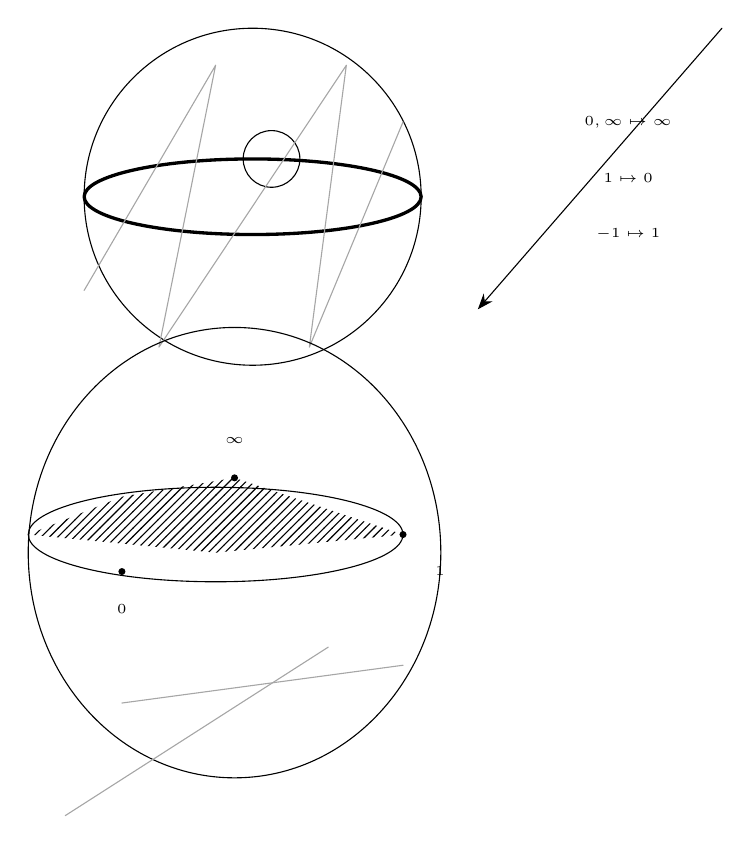
\begin{tikzpicture}[x=1mm,y=1mm,line cap=round,line join=round,font=\scriptsize]
\draw (33.3,-23.8) ellipse[x radius=21.4, y radius=21.4];
\draw[very thick] (33.3,-23.8) ellipse[x radius=21.4, y radius=4.8];
\draw (35.7,-19) circle[radius=3.6];
\draw[struck] (11.9,-35.7) -- (28.6,-7.1) -- (21.4,-42.9) -- (45.2,-7.1) -- (40.5,-42.9) -- (52.4,-14.3);
\draw (31,-69) ellipse[x radius=26.2, y radius=28.6];
\draw (28.6,-66.7) ellipse[x radius=23.8, y radius=6];
\node[pt] at (16.7,-71.4) {};
\node[pt] at (31,-59.5) {};
\node[pt] at (52.4,-66.7) {};
\fill[pattern=north east lines] (4.8,-66.7) -- (16.7,-61.9) -- (31,-59.5) -- (52.4,-66.7) -- (28.6,-69) -- cycle;
\node[inner sep=1pt] at (16.7,-76.2) {\tiny $0$};
\node[inner sep=1pt] at (31,-54.8) {\tiny $\infty$};
\node[inner sep=1pt] at (57.1,-71.4) {\tiny $1$};
\draw[struck] (9.5,-102.4) -- (42.9,-81);
\draw[struck] (16.7,-88.1) -- (52.4,-83.3);
\node[inner sep=1pt] at (81,-14.3) {\tiny $0,\infty\mapsto\infty$};
\node[inner sep=1pt] at (81,-21.4) {\tiny $1\mapsto 0$};
\node[inner sep=1pt] at (81,-28.6) {\tiny $-1\mapsto 1$};
\draw[-{Stealth[length=2mm]}] (92.9,-2.4) -- (61.9,-38.1);
\end{tikzpicture}
\end{document}
